\chapter{Rotations, spineurs et symétrie de couleur}

\section{Les rotations comme groupe}

Les rotations de l’espace sont des symétries qui agissent sur de nombreux types d’objets : les corps rigides, les vecteurs vitesse, les champs vectoriels et les états quantiques. Le vecteur ordinaire est le cas le plus simple pour commencer, car sa transformation se représente directement.

Les rotations peuvent aussi se composer. On fait tourner un objet d’un certain angle autour d’un axe, puis d’un autre angle autour d’un second axe. L’orientation finale équivaut à celle qu’aurait produite une rotation unique d’un certain angle autour d’un troisième axe. Le produit de deux rotations est donc une autre rotation.

Ce produit est une opération sur des transformations, et non une addition des vecteurs des axes. La première rotation transforme l’objet sur lequel agit la seconde. Si \(R_1\) est effectuée en premier et \(R_2\) en second, l’opération composée s’écrit \(R_2R_1\). Elle est elle-même une \(R_3\), même s’il peut être difficile de déterminer l’axe et l’angle de \(R_3\). Cette stabilité par composition est la première raison de considérer les rotations comme un groupe, plutôt que comme une simple liste de mouvements géométriques.

Commençons par décrire géométriquement une rotation. Choisissons un vecteur unitaire \(\hat{\boldsymbol n}\) dirigé selon l’axe de rotation et un angle \(\theta\). Nous adoptons la convention de la main droite. Une rotation de sens gauche d’angle \(\theta\) peut aussi s’écrire comme une rotation de sens droit d’angle \(-\theta\), ou comme une rotation de sens droit autour de \(-\hat{\boldsymbol n}\).

\begin{figure}[htbp]\centering
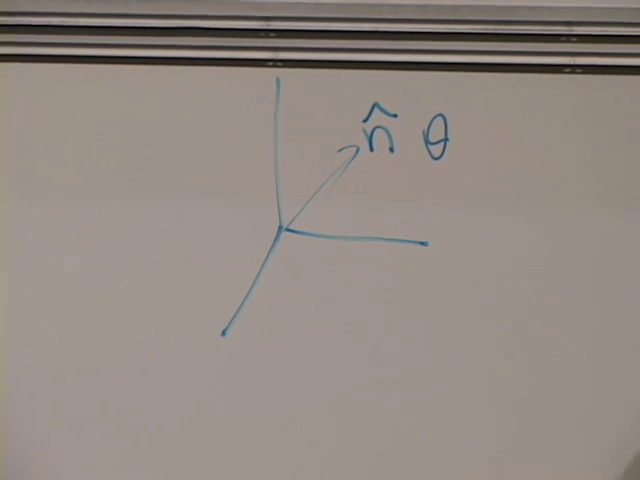
\includegraphics[width=0.58\textwidth]{lecture_03_figure_02.png}\caption{Un axe \(\hat{\boldsymbol n}\) et un angle \(\theta\) définissent une rotation spatiale.}\lectureframe{00:02:34}\end{figure}

Une direction sur la sphère unité nécessite deux paramètres, par exemple la longitude et la latitude. L’angle de rotation autour de cette direction en fournit un troisième. Les rotations forment donc une famille à trois paramètres. Nous ne nous préoccuperons pas encore des identifications globales dues aux angles qui diffèrent de \(2\pi\) ; c’est le nombre de paramètres locaux qui importe ici.

La description par l’axe et l’angle comporte une redondance. Inverser l’axe et l’angle donne la même opération, et les angles suffisamment grands peuvent être réduits modulo un tour complet. Rien de cela ne change le fait qu’au voisinage de l’identité, une rotation possède trois paramètres continus. Nous comparerons plus tard ce nombre local aux paramètres indépendants d’une représentation matricielle.

Vérifions maintenant l’une après l’autre les propriétés de groupe :
\begin{enumerate}\item \emph{Fermeture.} La composition de deux rotations successives donne une autre rotation.
\item \emph{Identité.} L’opération qui ne change rien est la rotation identité.
\item \emph{Inverse.} Une rotation d’angle \(\theta\) autour de \(\hat{\boldsymbol n}\) est annulée par une rotation d’angle \(-\theta\) autour du même axe.
\item \emph{Associativité.} Trois rotations successives vérifient
\[
(R_1R_2)R_3=R_1(R_2R_3).
\]\end{enumerate}

Les rotations ne commutent pas. Une rotation autour de l’axe \(x\) suivie d’une rotation autour de l’axe \(y\) donne généralement une orientation différente de celle obtenue en effectuant ces deux opérations dans l’ordre inverse :
\begin{equation}
R_x(\alpha)R_y(\beta)\ne R_y(\beta)R_x(\alpha).
\end{equation}
La différence est du second ordre lorsque les deux angles sont très petits, ce qui explique pourquoi les rotations infinitésimales peuvent sembler presque commutatives. Le groupe complet reste néanmoins non abélien.

On peut vérifier la non-commutativité sans aucune équation. Prenez un livre ou une boîte, repérez une face comme étant l’avant, puis effectuez une rotation de quatre-vingt-dix degrés autour de l’axe \(x\), suivie d’une rotation de quatre-vingt-dix degrés autour de l’axe \(y\). Revenez à l’orientation initiale et inversez l’ordre des rotations. La face repérée se retrouve orientée différemment. Pour de petits angles, l’écart est plus difficile à voir, mais il n’a pas disparu : il apparaît dès le produit des deux petits angles.

\begin{classroomqa}\audiencequestion{Ces rotations sont-elles successives plutôt que simultanées ?\lecturetimestamp{00:04:45}}\lecturerresponse{Oui. La multiplication dans un groupe signifie qu’une opération est suivie d’une autre. C’est précisément l’ordre de ces rotations successives qui peut empêcher la commutativité.}\end{classroomqa}

Voici notre premier groupe non abélien. L’application qui nous intéressera n’est pas la couleur d’un objet ordinaire, mais les états de couleur rouge, vert et bleu d’un quark. Il s’agit d’un système interne à trois états, dont les transformations intéressantes mélangent les trois couleurs. Les rotations ordinaires fournissent un exemple familier de l’action d’un groupe continu par l’intermédiaire de matrices.

Un groupe est abstrait en lui-même. Pour l’utiliser en physique, nous devons préciser sur quels objets il agit. Une {représentation} associe un opérateur ou une matrice à chaque élément du groupe, de sorte que la multiplication des éléments du groupe soit reproduite par la multiplication des matrices associées. Différents objets physiques peuvent porter différentes représentations d’un même groupe. Les vecteurs, les états de spin un et les états de spin un demi en fourniront trois exemples.

\section{La représentation vectorielle tridimensionnelle}

Considérons un vecteur ordinaire de composantes
\begin{equation}
\boldsymbol V=(V_x,V_y,V_z),\qquad V_i,\quad i=1,2,3.
\end{equation}
On peut faire tourner le vecteur physique en gardant les axes fixes, ou faire tourner les axes de coordonnées en gardant le vecteur fixe. Les conventions diffèrent, mais dans les deux descriptions, les composantes sont mélangées par une matrice \(3\times3\). Pour chaque couple axe-angle \((\hat{\boldsymbol n},\theta)\), écrivons
\begin{equation}
V_i'=R_{ij}(\hat{\boldsymbol n},\theta)V_j,
\label{eq:l3-vector-rotation}
\end{equation}
où l’on somme sur tout indice répété.

L’indice répété \(j\) est un indice muet. L’équation~\eqref{eq:l3-vector-rotation} signifie explicitement
\begin{equation}
V_i'=R_{i1}V_1+R_{i2}V_2+R_{i3}V_3
\end{equation}
pour chaque composante de sortie \(i\). L’indice libre \(i\) désigne la composante calculée ; l’indice répété \(j\) est muet et peut être renommé sans modifier l’équation. Distinguer ces deux rôles permet d’éviter la plupart des erreurs d’indices dans l’argument de conservation de la longueur.

\begin{figure}[htbp]\centering
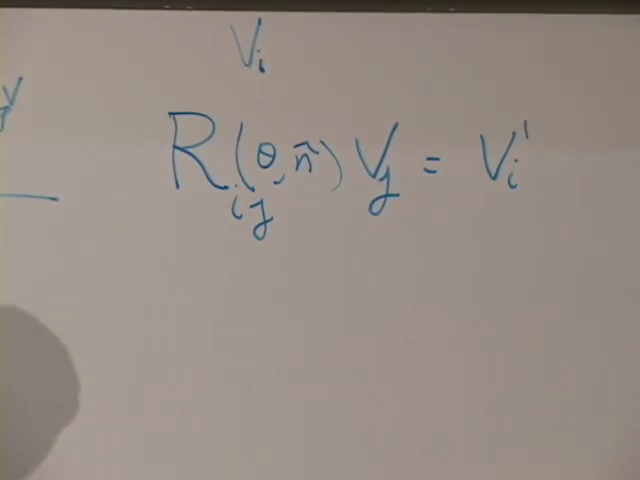
\includegraphics[width=0.68\textwidth]{lecture_03_figure_03.png}\caption{Une matrice de rotation transforme les composantes du vecteur initial en celles du vecteur après rotation.}\lectureframe{00:07:41}\end{figure}

Une rotation véritable conserve la longueur. Pour l’instant, \(V_i\) et \(R_{ij}\) sont réels, donc
\begin{equation}
V_i'V_i'=V_iV_i
\end{equation}
pour tout vecteur. Pour mettre en évidence la condition matricielle, écrivons la même transformation avec des indices muets différents :
\begin{equation}
V_i'=R_{ij}V_j,\qquad V_i'=R_{ik}V_k.
\end{equation}
En multipliant puis en sommant sur \(i\), on obtient
\begin{align}
V_i'V_i'
 &=R_{ij}V_jR_{ik}V_k\\
 &=R_{ij}R_{ik}V_jV_k.
\end{align}
Cela vaut \(V_jV_j\) pour tout choix de \(V\) seulement si
\begin{equation}
R_{ij}R_{ik}=\delta_{jk}.
\label{eq:l3-orthogonality-index}
\end{equation}
En notation matricielle,
\begin{equation}
R^TR=\boldsymbol 1,
\label{eq:l3-orthogonal}
\end{equation}
et donc
\begin{equation}
R^{-1}=R^T.
\end{equation}
La transposition échange simplement les lignes et les colonnes.

Pourquoi le coefficient doit-il être \(\delta_{jk}\) ? Le delta de Kronecker impose \(j=k\) dans la somme :
\begin{equation}
\delta_{jk}V_jV_k=V_1^2+V_2^2+V_3^2.
\end{equation}
Si \(R_{ij}R_{ik}\) différait de \(\delta_{jk}\), une direction ou un terme croisé \(V_jV_k\) modifierait la longueur. Comme l’égalité doit être vérifiée pour tout vecteur possible, et pas seulement pour un vecteur choisi, le coefficient matriciel lui-même doit être égal à l’identité.

L’équation~\eqref{eq:l3-orthogonal} est la condition d’orthogonalité qui définit cette représentation matricielle réelle. La multiplication des matrices reproduit la table de multiplication des rotations spatiales. Ce n’est pas la seule représentation du groupe des rotations : c’est simplement la plus facile à visualiser.

La relation d’inversion a une signification géométrique immédiate. On peut annuler une rotation sans résoudre une nouvelle équation matricielle : il suffit d’échanger les lignes et les colonnes. Si \(R_1\) et \(R_2\) représentent deux rotations, alors \(R_2R_1\) représente leur action successive et est encore orthogonale. Les opérations matricielles préservent donc les mêmes propriétés de fermeture, d’identité, d’inverse et d’associativité que celles établies géométriquement.

\section{Spin un et représentation vectorielle}

La représentation tridimensionnelle agit aussi sur les états quantiques. Une particule de spin un possède trois projections de spin possibles :
\begin{equation}
m=+1,\quad 0,\quad -1.
\end{equation}
Son état de spin est donc une colonne à trois composantes d’amplitudes de probabilité. Faire tourner la particule, ou changer l’orientation du champ magnétique qui définit l’axe de spin, mélange ces trois amplitudes selon une représentation tridimensionnelle du groupe des rotations.

Le nombre d’états de spin suit la règle bien connue \(2s+1\). Le spin zéro a un état, le spin un demi en a deux, le spin un en a trois et le spin trois demis en a quatre. La dimension du vecteur d’état varie donc avec le spin. Une même rotation physique doit être représentée par des matrices de tailles différentes lorsqu’elle agit sur ces différents espaces d’états.

Pour une particule de spin un, choisissons la base
\begin{equation}
\lvert 1,+1\rangle,qquad
\lvert 1,0\rangle,qquad
\lvert 1,-1\rangle.
\end{equation}
Un état s’écrit
\begin{equation}
\lvert\psi\rangle
=c_{+}\lvert1,+1\rangle+c_0\lvert1,0\rangle+c_{-}\lvert1,-1\rangle.
\end{equation}
La rotation de l’appareil ne crée pas un quatrième état de spin ; elle mélange entre eux les trois coefficients \(c_+,c_0,c_-\). L’opérateur de rotation correspondant doit donc être une matrice \(3\times3\).

Pour le spin un, cette représentation se transforme comme un vecteur spatial ordinaire. C’est le sens précis de l’expression \emph{particule vectorielle} pour désigner une particule de spin un : ses trois amplitudes de spin et les trois composantes d’un vecteur obéissent à la même loi de rotation. Il n’est pas nécessaire d’imaginer l’état quantique comme une flèche au sens littéral ; l’énoncé porte sur la manière dont ses composantes se mélangent.

Cette correspondance n’est pas fortuite. Un vecteur à trois composantes et un état de spin un portent des représentations tridimensionnelles équivalentes du groupe des rotations. L’expression {particule vectorielle} résume cette propriété de transformation. Elle ne prétend pas qu’un état de polarisation quantique soit une petite flèche rigide cachée dans la particule.

\section{Symétries discrètes et continues}

Avant d’aborder le spin un demi, il est utile de distinguer deux grandes catégories de groupes. Une réflexion fournit un exemple discret simple. Il y a l’identité et la réflexion \(P\) ; on effectue la symétrie ou on ne l’effectue pas. En revanche, une phase
\begin{equation}
e^{i\phi}
\end{equation}
dépend continûment de \(\phi\), tout comme une rotation spatiale dépend continûment de son axe et de son angle. Ces groupes continus sont appelés \emph{groupes de Lie}, d’après Sophus Lie ; le nom se prononce \emph{Li}. Les symétries continues seront au cœur de notre étude, même si les symétries discrètes restent importantes.

Pour le groupe de réflexion à deux éléments,
\begin{equation}
P^2=1.
\end{equation}
il n’existe aucune valeur de réflexion continûment ajustable entre \(1\) et \(P\). Le groupe des phases est différent : il existe continûment de nombreuses phases entre \(e^{i\phi_1}\) et \(e^{i\phi_2}\). Les rotations spatiales ont le même caractère continu, mais, contrairement à \(U(1)\), elles sont non abéliennes.

Le spin zéro fournit la représentation la plus simple du groupe des rotations. Un état de spin zéro est inchangé par toute rotation ; chaque élément du groupe est donc représenté par l’identité unidimensionnelle :
\begin{equation}
D^{(0)}(R)=1.
\end{equation}
Le groupe lui-même contient toujours une infinité de rotations ; c’est la représentation agissant sur l’état de spin zéro qui est triviale.

Cette distinction entre un groupe et l’une de ses représentations est essentielle. Le groupe des rotations ne se réduit pas à un groupe à un seul élément lorsqu’il agit sur un scalaire. Chacun de ses éléments est plutôt représenté par le même nombre \(1\) sur ce scalaire particulier.

\section{État général de spin un demi}

Un système de spin un demi possède deux états de base. Par rapport à un axe \(z\) choisi,
\begin{equation}
\lvert\uparrow\rangle=
\begin{pmatrix}1\\0\end{pmatrix},
\qquad
\lvert\downarrow\rangle=
\begin{pmatrix}0\\1\end{pmatrix}.
\end{equation}
Un état général est un spineur à deux composantes :
\begin{equation}
\lvert\psi\rangle=
\begin{pmatrix}\alpha_1\\\alpha_2\end{pmatrix},
\qquad
|\alpha_1|^2+|\alpha_2|^2=1.
\label{eq:l3-spinor}
\end{equation}
Ses composantes sont complexes. Le choix \((\alpha_1,\alpha_2)=(1,0)\) correspond au spin vers le haut, et \((0,1)\) au spin vers le bas. Une combinaison générale normalisée décrit un spin polarisé selon une autre direction.

Les termes {vers le haut} et {vers le bas} n’ont de sens qu’une fois un axe choisi. Ici, cet axe est \(z\). Un autre axe de mesure définit une autre paire d’états de base, et un état bien défini vers le haut selon un axe apparaît généralement comme une superposition dans une autre base. Faire tourner le spin physique ou les axes de référence modifie les coefficients en conséquence.

Deux amplitudes complexes contiennent quatre paramètres réels. La normalisation en élimine un, et la phase globale sans effet physique en élimine un autre ; il reste deux paramètres réels. C’est exactement le nombre nécessaire pour choisir une direction sur une sphère. Pour étudier les rotations, il n’est pas nécessaire de dériver la correspondance explicite entre \((\alpha_1,\alpha_2)\) et cette direction.

La phase globale est éliminée parce que
\begin{equation}
\begin{pmatrix}\alpha_1\\\alpha_2\end{pmatrix}
\quad\hbox{and}\quad
e^{i\chi}
\begin{pmatrix}\alpha_1\\\alpha_2\end{pmatrix}
\end{equation}
représentent le même rayon physique. La normalisation fixe la probabilité totale, et non une direction dans l’espace euclidien ordinaire. Après ces deux identifications, les deux paramètres restants peuvent être considérés comme les angles polaire et azimutal de la direction de polarisation du spin.

Lorsque le spin subit une rotation, son état devient
\begin{equation}
\alpha_i'=U_{ij}\alpha_j,
\qquad
\begin{pmatrix}\alpha_1'\\\alpha_2'\end{pmatrix}
=
\begin{pmatrix}
U_{11}&U_{12}\\
U_{21}&U_{22}
\end{pmatrix}
\begin{pmatrix}\alpha_1\\\alpha_2\end{pmatrix}.
\label{eq:l3-spinor-transform}
\end{equation}
Les rotations spatiales possèdent donc une représentation matricielle de dimension deux agissant sur les spineurs. Cette représentation présente une ambiguïté globale à deux valeurs que nous examinerons plus tard ; localement, les matrices ont les propriétés de transformation nécessaires pour la suite.

La paire transformée \((\alpha_1',\alpha_2')\) doit encore être un état quantique admissible. La première question à propos de \(U\) ne porte donc pas sur sa formule explicite en fonction de l’axe et de l’angle, mais sur la condition qui garantit la conservation de la normalisation de tout spineur d’entrée.

\section{Conservation de la probabilité et matrices unitaires}

Une rotation doit transformer un état normalisé en un autre état normalisé :
\begin{equation}
\alpha_i^*\alpha_i=\alpha_i'^*\alpha_i'=1.
\end{equation}
En substituant l’équation~\eqref{eq:l3-spinor-transform},
\begin{align}
\alpha_i'^*\alpha_i'
 &=(U_{ij}\alpha_j)^*(U_{ik}\alpha_k)\\
 &=\alpha_j^*U_{ij}^*U_{ik}\alpha_k.
\end{align}
L’analogue de la condition imposée au vecteur réel est donc
\begin{equation}
(U^T)^*U=\boldsymbol 1.
\end{equation}
La transposée suivie de la conjugaison complexe est l’adjointe hermitienne :
\begin{equation}
U^\dagger=(U^T)^*,
\end{equation}
La condition de conservation de la normalisation s’écrit alors
\begin{equation}
U^\dagger U=\boldsymbol 1.
\label{eq:l3-unitarity}
\end{equation}

La conjugaison complexe est la seule modification essentielle par rapport au calcul sur les vecteurs réels. Pour un vecteur réel, \(V_iV_i\) est une longueur. Pour un spineur, \(\alpha_i^*\alpha_i\) est une probabilité. La conjugaison complexe est nécessaire pour rendre cette probabilité réelle et non négative ; la transposition est donc remplacée par l’adjonction hermitienne.

L’équation~\eqref{eq:l3-unitarity} donne aussi immédiatement l’inverse :
\begin{equation}
U^{-1}=U^\dagger.
\end{equation}
La rotation inverse conserve donc la même norme de probabilité. Comme pour les matrices de rotation ordinaires, le produit de matrices unitaires reste unitaire ; la représentation respecte ainsi la multiplication du groupe.

\begin{figure}[htbp]\centering
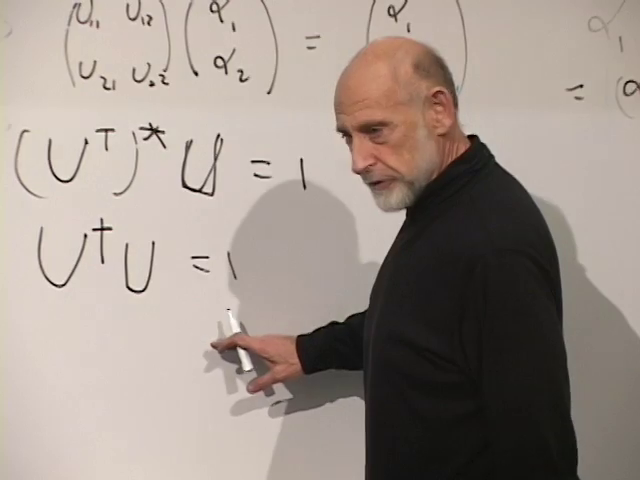
\includegraphics[width=0.62\textwidth]{lecture_03_figure_04.png}\caption{La matrice de rotation du spineur vérifie \(U^\dagger U=\boldsymbol 1\).}\lectureframe{00:27:41}\end{figure}

Les matrices qui vérifient l’équation~\eqref{eq:l3-unitarity} sont unitaires. Une matrice complexe générale \(2\times2\) possède au départ huit paramètres réels. L’unitarité impose une équation matricielle \(2\times2\) qui fournit quatre contraintes réelles indépendantes ; il reste donc quatre paramètres. Une rotation spatiale n’en possède que trois. Il faut une restriction supplémentaire pour isoler la représentation des rotations sur les spineurs de l’ensemble \(U(2)\).

On peut aussi voir les quatre contraintes en considérant les deux colonnes de \(U\) comme deux vecteurs complexes. Chaque colonne doit être de norme unitaire, ce qui fournit deux conditions réelles, et les colonnes doivent être orthogonales, ce qui fournit une condition complexe, soit deux conditions réelles. Cela fait quatre au total. Le quatrième paramètre restant dans \(U(2)\) se révélera être une phase globale du déterminant, et non une nouvelle rotation spatiale.

\section{Déterminant unitaire et \texorpdfstring{\(SU(2)\)}{SU(2)}}

La condition supplémentaire est
\begin{equation}
\det U=1.
\label{eq:l3-det-one}
\end{equation}
Elle est compatible avec la multiplication du groupe, car
\begin{equation}
\det(AB)=\det A\,\det B.
\end{equation}
Le produit de deux matrices unitaires de déterminant un est encore de déterminant un, et l’identité a un déterminant égal à un. Ces matrices forment un sous-groupe fermé.

L’inverse appartient lui aussi au sous-groupe. Si \(\det U=1\), alors
\begin{equation}
\det U^{-1}=\frac{1}{\det U}=1.
\end{equation}
Imposer un déterminant égal à un ne supprime donc pas l’identité, ne compromet pas la fermeture et ne fait perdre aucun inverse. Cette condition sélectionne de manière cohérente un groupe qui possède un paramètre continu de moins.

L’unitarité seule implique
\begin{equation}
\det(U^\dagger U)=
(\det U)^*\det U
=|\det U|^2=1.
\end{equation}
Elle n’impose pas que \(\det U\) soit égal à \(+1\) ou à \(-1\). Le déterminant d’une matrice unitaire générale peut être une phase quelconque :
\begin{equation}
\det U=e^{i\phi},
\qquad
\det U^\dagger=e^{-i\phi}.
\end{equation}
La condition~\eqref{eq:l3-det-one} fixe cette phase autrement libre et élimine un paramètre réel.

\begin{classroomqa}\audiencequestion{La condition \(U^\dagger U=\boldsymbol 1\), sans imposer un déterminant égal à un, oblige-t-elle \(\det U^\dagger\) à être égal à \(\det U\) ou à valoir uniquement \(+1\) ou \(-1\) ?\lecturetimestamp{00:31:21}}\lecturerresponse{Non. Les deux déterminants sont des conjugués complexes. Ils peuvent être égaux à \(e^{i\phi}\) et \(e^{-i\phi}\), dont le produit vaut un. La condition spéciale unitaire les fixe alors tous deux à un.}\end{classroomqa}

Les matrices unitaires \(n\times n\) forment le groupe \(U(n)\). Pour \(n=1\), une matrice unitaire se réduit simplement à la phase \(e^{i\phi}\), ce qui donne \(U(1)\). Le sous-groupe de déterminant un est le \emph{groupe spécial unitaire},
\begin{equation}
SU(n)=\{U\in U(n):\det U=1\}.
\end{equation}
Le spineur à deux composantes est soumis à l’action de \(SU(2)\), un groupe à trois paramètres.

La notation indique les deux restrictions : \(U\) signifie unitaire, tandis que \(S\) signifie spécial, c’est-à-dire de déterminant un. Ces groupes spéciaux unitaires reviennent souvent, car ils préservent un produit scalaire complexe tout en excluant la phase commune indépendante portée par le déterminant.

Localement, \(SU(2)\) possède l’algèbre des rotations et la structure de multiplication nécessaires pour faire tourner les états de spin un demi. Globalement, il faut garder à l’esprit la subtilité laissée en suspens : \(SU(2)\) est le revêtement double du groupe ordinaire des rotations \(SO(3)\) ; deux éléments de \(SU(2)\) correspondent donc à une seule rotation spatiale. \editorialnote{La formulation par revêtement double précise l’ambiguïté à deux valeurs mentionnée, mais non développée, dans la source.}

\section{Rotations infinitésimales et matrices de Pauli}

\begin{classroomqa}\audiencequestion{À quel moment les matrices de spin, ou matrices de Pauli, interviennent-elles dans cette construction ?\lecturetimestamp{00:33:16}}\lecturerresponse{Elles apparaissent lorsqu’on prend un élément du groupe très proche de l’identité, ce qui correspond à une rotation d’angle très petit. Ce sont les générateurs de ces rotations infinitésimales.}\end{classroomqa}

Commençons par
\begin{equation}
U=\boldsymbol 1+\epsilon M+O(\epsilon^2),
\label{eq:l3-small-u-anti}
\end{equation}
où \(\epsilon\) est réel et petit. Alors
\begin{equation}
U^\dagger=\boldsymbol 1+\epsilon M^\dagger+O(\epsilon^2),
\end{equation}
et l’unitarité donne
\begin{align}
U^\dagger U
 &=\boldsymbol 1+\epsilon(M^\dagger+M)+O(\epsilon^2).
\end{align}
Au premier ordre,
\begin{equation}
M^\dagger=-M.
\end{equation}
La matrice \(M\) de l’équation~\eqref{eq:l3-small-u-anti} est donc anti-hermitienne.

On ne conserve que les termes linéaires en \(\epsilon\). Le produit \(\epsilon^2M^\dagger M\) est négligé, car il est du second ordre. C’est l’avantage de travailler au voisinage de l’identité : les conditions non linéaires du groupe deviennent des conditions linéaires sur ses générateurs.

Il est plus pratique d’extraire un facteur \(i\) :
\begin{equation}
U=\boldsymbol 1+i\epsilon H+O(\epsilon^2).
\label{eq:l3-small-u-herm}
\end{equation}
La conjugaison complexe transforme \(i\) en \(-i\), donc
\begin{equation}
U^\dagger=\boldsymbol 1-i\epsilon H^\dagger+O(\epsilon^2).
\end{equation}
Or
\begin{equation}
U^\dagger U
=\boldsymbol 1+i\epsilon(H-H^\dagger)+O(\epsilon^2),
\end{equation}
L’unitarité au premier ordre impose alors
\begin{equation}
H^\dagger=H.
\end{equation}
Une fois le facteur \(i\) extrait, le générateur est hermitien.

La multiplication par \(i\) n’a pas modifié les matrices infinitésimales admissibles ; elle a seulement changé la convention utilisée pour nommer le générateur. En physique, on choisit généralement des générateurs hermitiens parce que leurs valeurs propres sont réelles et que les observables correspondantes, comme le moment cinétique, sont hermitiennes.

La condition de déterminant un impose que la trace soit nulle\editorialnote{\(A_{11}+A_{22}=\operatorname{tr}A\)}. Pour une matrice \(2\times2\) \(A\) petite,
\begin{equation}
\det(\boldsymbol 1+A)
=
\det
\begin{pmatrix}
1+A_{11}&A_{12}\\
A_{21}&1+A_{22}
\end{pmatrix}.
\end{equation}
En développant,
\begin{align}
\det(\boldsymbol 1+A)
 &=(1+A_{11})(1+A_{22})-A_{12}A_{21}\\
 &=1+A_{11}+A_{22}+O(A^2)\\
 &=1+\operatorname{tr}A+O(A^2).
\end{align}
Appliquons ce résultat à \(A=i\epsilon H\) :
\begin{equation}
\det U=1+i\epsilon\,\operatorname{tr}H+O(\epsilon^2).
\end{equation}
Par conséquent, \(\det U=1\) impose
\begin{equation}
\operatorname{tr}H=0.
\end{equation}
La condition de trace élimine précisément le générateur proportionnel à la matrice identité. Une matrice hermitienne générale \(2\times2\) possède quatre paramètres réels : deux éléments diagonaux réels et un élément hors diagonale complexe. Sa trace fixe une combinaison réelle ; il en reste trois. Cela correspond aux trois axes autour desquels peut s’effectuer une rotation spatiale infinitésimale.

Les générateurs infinitésimaux de \(SU(2)\) sont donc des matrices hermitiennes sans trace \(2\times2\). Les trois matrices de Pauli en forment une base :
\begin{equation}
\begin{aligned}
\sigma_x&=
\begin{pmatrix}0&1\\1&0\end{pmatrix},
&
\sigma_y&=
\begin{pmatrix}0&-i\\i&0\end{pmatrix},
\\[0.4em]
\sigma_z&=
\begin{pmatrix}1&0\\0&-1\end{pmatrix}.
\end{aligned}
\end{equation}
Tout générateur peut s’écrire
\begin{equation}
H=a_x\sigma_x+a_y\sigma_y+a_z\sigma_z.
\end{equation}
Une petite rotation autour de l’axe \(x\) sélectionne \(\sigma_x\) ; une rotation autour de l’axe \(y\) sélectionne \(\sigma_y\) ; une rotation autour de tout autre axe sélectionne la combinaison linéaire correspondante. Dans les unités où \(\hbar=1\), les opérateurs de spin sont
\begin{equation}
S_i=\frac{\sigma_i}{2}.
\end{equation}

Par exemple, un axe à mi-chemin entre \(x\) et \(y\) utilise un générateur proportionnel à
\begin{equation}
\frac{\sigma_x+\sigma_y}{\sqrt2}.
\end{equation}
La direction du vecteur de coefficients \((a_x,a_y,a_z)\) sélectionne l’axe de rotation, tandis que sa norme, combinée à \(\epsilon\), détermine le petit angle. Voilà le lien entre les matrices de spin rencontrées dans les relations de commutation du moment cinétique et les opérateurs de rotation finis. En particulier,
\begin{equation}
[S_x,S_y]=iS_z
\end{equation}
et les relations cycliques correspondantes encodent la non-commutativité déjà observée géométriquement. La rotation finie usuelle s’obtient en exponentiant le générateur infinitésimal\editorialnote{},
\begin{equation}
U(\hat{\boldsymbol n},\theta)
=\exp\left(-\frac{i\theta}{2}\,
\hat{\boldsymbol n}\cdot\boldsymbol\sigma\right).
\end{equation}\section{Un espace de couleur à trois états}

Nous pourrons combiner les représentations plus tard. Quittons maintenant le spin spatial pour revenir à la couleur des quarks. Un quark a toujours un spin un demi, mais sa couleur est un degré de liberté indépendant à trois états :
\begin{equation}
\lvert r\rangle,\qquad
\lvert g\rangle,\qquad
\lvert b\rangle.
\end{equation}
Un état général de couleur s’écrit
\begin{equation}
\begin{aligned}
\lvert q\rangle_{\mathrm{color}}
={}&
\alpha_r\lvert r\rangle
+\alpha_g\lvert g\rangle
+\alpha_b\lvert b\rangle,
\\
&|\alpha_r|^2+|\alpha_g|^2+|\alpha_b|^2=1.
\end{aligned}
\end{equation}
De manière équivalente,
\begin{equation}
q=
\begin{pmatrix}
\alpha_r\\
\alpha_g\\
\alpha_b
\end{pmatrix}.
\end{equation}
Les carrés des modules sont les probabilités d’obtenir le rouge, le vert ou le bleu dans une base de couleur choisie. La même notation en triplet permet de rassembler trois opérateurs de champ de quark :
\begin{equation}
\psi=
\begin{pmatrix}
\psi_r\\
\psi_g\\
\psi_b
\end{pmatrix}.
\end{equation}

Il faut garder le spin et la couleur conceptuellement distincts. L’étiquette de spin indique comment l’état se transforme sous l’effet des rotations de l’espace physique. L’étiquette de couleur indique comment il se transforme sous une symétrie interne qui ne fait pas tourner le laboratoire. Un état de quark porte les deux étiquettes, même si la discussion présente omet le spin pour se concentrer sur la couleur.

Écrire trois opérateurs de champ dans une même colonne ne relève pas seulement de la mise en ordre. Cela permet d’exprimer la symétrie par une seule équation matricielle. Une transformation peut convertir un champ rouge en une combinaison linéaire de champs rouge, vert et bleu, tout comme une rotation spatiale transforme une composante d’un vecteur en une combinaison linéaire de ses autres composantes.

On peut d’abord envisager des transformations discrètes qui échangent deux couleurs. La symétrie plus vaste contient des mélanges continus des trois couleurs. Une matrice d’échange simple peut nécessiter une phase supplémentaire pour que son déterminant soit égal à un ; l’échange s’inscrit alors dans le groupe spécial unitaire.

Pour deux états de base, l’échange direct est représenté par
\begin{equation}
X=
\begin{pmatrix}0&1\\1&0\end{pmatrix},
\qquad
\det X=-1.
\end{equation}
La multiplication de toute la matrice par \(i\) donne
\begin{equation}
\det(iX)=i^2\det X=1.
\end{equation}
L’échange discret peut donc apparaître comme un élément particulier du groupe continu plus vaste, à condition de choisir la phase de façon cohérente.

\begin{classroomqa}\audiencequestion{Une matrice qui échange simplement deux états de base a-t-elle un déterminant incompatible avec \(SU(2)\) ?\lecturetimestamp{00:43:46}}\lecturerresponse{L’échange direct a pour déterminant \(-1\). Un facteur \(i\) convenablement choisi fournit un représentant de déterminant un ; l’échange peut donc être inclus dans les transformations continues du groupe spécial unitaire.}\end{classroomqa}

\section{\texorpdfstring{\(SU(3)\)}{SU(3)} et les huit générateurs de couleur}

La transformation continue de couleur est
\begin{equation}
\begin{aligned}
q'&=Uq,
&
U^\dagger U&=\boldsymbol 1,
\\
\det U&=1,
&
U&\in SU(3).
\end{aligned}
\label{eq:l3-su3-action}
\end{equation}
Les mathématiques reprennent la même construction spéciale unitaire que pour les spineurs, mais ici \(U\) est une matrice \(3\times3\). Il ne s’agit pas d’une rotation de l’espace physique, mais d’une rotation dans l’espace interne des couleurs.

L’unitarité préserve la normalisation de l’état de couleur :
\begin{equation}
q^\dagger q
=|\alpha_r|^2+|\alpha_g|^2+|\alpha_b|^2.
\end{equation}
La condition de déterminant un élimine la direction de phase commune \(U(1)\) parmi les mélanges continus. Les matrices obtenues peuvent effectuer des échanges simples, des changements de phase relative et des superpositions réellement continues, tout en appartenant à un même groupe fermé.

Le décompte des paramètres est immédiat. Une matrice complexe \(3\times3\) possède neuf entrées complexes, soit dix-huit paramètres réels. L’équation matricielle \(U^\dagger U=\boldsymbol 1\) impose neuf conditions réelles. La condition de déterminant un en élimine encore une :
\begin{equation}
\dim SU(3)=18-9-1=8.
\end{equation}
Ainsi, \(SU(3)\) possède huit générateurs infinitésimaux indépendants.

On peut aussi interpréter les neuf conditions réelles d’unitarité en considérant les colonnes de \(U\). Trois colonnes complexes doivent chacune être de norme unitaire, et toute paire doit être orthogonale. Ces conditions éliminent neuf des dix-huit paramètres réels initiaux. La phase du déterminant en élimine un dixième ; il en reste huit. C’est l’analogue, pour trois états, du décompte \(8-4-1=3\) pour \(SU(2)\).

L’apparition du nombre huit correspond au même fait qui conduit finalement à huit espèces de gluons. Dire qu’il n’y a pas neuf gluons parce que la contrainte sur le déterminant a éliminé une direction n’est qu’un moyen mnémotechnique. Plus précisément, les neuf matrices couleur-anticouleur se décomposent en une direction singulet de couleur, proportionnelle à l’identité, et huit directions sans trace. Les huit générateurs sans trace forment la structure adjointe de couleur portée par les gluons de la QCD.\editorialnote{La formulation en un singulet et un octet est la version précise standard de la remarque volontairement heuristique de la source sur le déterminant ; la construction du champ de jauge est abordée plus loin.}

À ce stade, le lien avec les huit gluons est un repère, et non encore une dérivation complète. Pour obtenir des particules de jauge, il faut promouvoir la symétrie de couleur au rang de symétrie locale et déterminer les champs compensateurs. Le décompte des paramètres a déjà montré qu’il existe huit directions indépendantes selon lesquelles une transformation de couleur \(SU(3)\) peut s’écarter de l’identité.

\section{La symétrie de couleur impose des contraintes à la QCD}

L’énoncé fondamental de symétrie est que la physique reste invariante sous la transformation de couleur de l’équation~\eqref{eq:l3-su3-action}. C’est la symétrie interne centrale de la chromodynamique quantique. Le mélange des composantes de couleur est formellement analogue au mélange des amplitudes de spin haut et de spin bas ; ces transformations de spineurs sont, à leur tour, liées aux rotations des directions spatiales, mais il ne faut pas confondre ces trois espaces.

Dire que la couleur est une symétrie signifie qu’un changement de base de couleur ne modifie pas les prédictions physiques. Rouge, vert et bleu sont des noms commodes pour trois vecteurs de base, et non trois pigments observables. Une rotation simultanée \(SU(3)\) des composantes de couleur doit laisser inchangée la forme des lois. Cette invariance n’est pas un simple choix esthétique : elle constitue le principe organisateur de la QCD.

La symétrie restreint le lagrangien. Dans l’exemple antérieur \(U(1)\), l’invariance sous une transformation de phase commune imposait que les termes autorisés contiennent des facteurs équilibrés d’un champ et de son conjugué. En QCD, chaque terme doit de même être invariant sous la transformation \(SU(3)\) de couleur. Cette exigence a des conséquences sur les interactions, les quantités conservées et la forme du champ de gluon.

Supposons qu’un terme proposé porte un indice de couleur libre. Sous l’action de l’équation~\eqref{eq:l3-su3-action}, cet indice subit une rotation ; le terme ne peut donc pas être invariant à lui seul. Les termes autorisés doivent contracter les indices de couleur en combinaisons invariantes, ou faire intervenir des champs de jauge dont les transformations compensent le changement. C’est là l’effet concret du principe de symétrie : il exclut les couplages arbitraires et organise les interactions qui subsistent.

La construction complète de la QCD exige une étape supplémentaire : il faut permettre à la transformation de couleur de varier d’un point à l’autre, et le champ de jauge doit compenser cette variation locale.\editorialnote{La localisation de la symétrie de couleur est le complément standard de la discussion sur la symétrie globale \(SU(3)\) en théorie de jauge ; elle n’est pas développée dans ce cours.} Cette étape viendra ensuite. Pour l’instant, la structure essentielle est en place : un triplet de couleur sur lequel agit une symétrie unitaire spéciale à trois états, dotée de huit générateurs.

Le calcul est allé aussi loin dans la théorie des groupes qu’il est nécessaire pour le moment. Nous sommes partis de rotations que l’on peut représenter dans l’espace ordinaire, avons considéré les matrices agissant sur les vecteurs et les spineurs, puis avons repris le même raisonnement dans un espace interne de couleur. L’étape suivante pourra revenir à la physique des particules en s’appuyant sur ce cadre mathématique, sans demander au formalisme de porter à lui seul toute l’histoire physique.